% ============================================================
%  India NLP Quant Research Terminal — Academic Project Report
%  IIT Mandi  |  May 2025
%  Compile:  pdflatex report.tex  (run twice for ToC)
% ============================================================
\documentclass[12pt, a4paper]{article}

% ── Packages ────────────────────────────────────────────────
\usepackage[top=2.5cm, bottom=2.5cm, left=3cm, right=2.5cm]{geometry}
\usepackage[T1]{fontenc}
\usepackage[utf8]{inputenc}
\usepackage{mathptmx}          % Times-compatible math + text font
\usepackage{microtype}
\usepackage{setspace}
\usepackage{titlesec}
\usepackage{titling}
\usepackage{fancyhdr}
\usepackage{graphicx}
\usepackage{amsmath, amssymb}
\usepackage{booktabs}
\usepackage{array}
\usepackage{xcolor}
\usepackage{hyperref}
\usepackage{listings}
\usepackage{caption}
\usepackage{subcaption}
\usepackage{tocloft}
\usepackage{mdframed}
\usepackage{enumitem}
\usepackage{float}
\usepackage{tikz}
\usetikzlibrary{shapes.geometric, arrows.meta, positioning, fit, backgrounds}
\usepackage{pgfplots}
\pgfplotsset{compat=1.18}

% ── Paragraph and spacing control ───────────────────────────
\setlength{\parindent}{1.2em}
\setlength{\parskip}{4pt plus 1pt}
\setlength{\baselineskip}{14pt}
\setstretch{1.15}

% ── Colors ──────────────────────────────────────────────────
\definecolor{IITBlue}{RGB}{0,51,102}
\definecolor{IITLightBlue}{RGB}{0,102,204}
\definecolor{CodeGray}{RGB}{245,245,245}
\definecolor{CommentGreen}{RGB}{0,128,0}

% ── Hyperref Setup ───────────────────────────────────────────
\hypersetup{
    colorlinks=true,
    linkcolor=IITBlue,
    citecolor=IITBlue,
    urlcolor=IITLightBlue,
    pdftitle={India NLP Quant Research Terminal},
    pdfauthor={Aditi Gupta, Siddhi Pogakwar, Anamika Godara, Shubh Sahu}
}

% ── Section Formatting ──────────────────────────────────────
\titleformat{\section}{\large\bfseries\color{IITBlue}}{\thesection}{1em}{}[\titlerule]
\titleformat{\subsection}{\normalsize\bfseries\color{IITLightBlue}}{\thesubsection}{1em}{}
\titleformat{\subsubsection}{\normalsize\bfseries}{\thesubsubsection}{1em}{}

% Tighten section vertical spacing
\titlespacing*{\section}      {0pt}{14pt}{6pt}
\titlespacing*{\subsection}   {0pt}{10pt}{4pt}
\titlespacing*{\subsubsection}{0pt}{8pt}{2pt}

% ── Header / Footer ─────────────────────────────────────────
\pagestyle{fancy}
\fancyhf{}
\fancyhead[L]{\small\color{IITBlue} India NLP Quant Research Terminal}
\fancyhead[R]{\small\color{IITBlue} IIT Mandi}
\fancyfoot[C]{\thepage}
\renewcommand{\headrulewidth}{0.4pt}

% ── Code Listing Style ──────────────────────────────────────
\lstset{
    backgroundcolor=\color{CodeGray},
    basicstyle=\ttfamily\scriptsize,
    keywordstyle=\color{IITBlue}\bfseries,
    commentstyle=\color{CommentGreen}\itshape,
    stringstyle=\color{red},
    frame=single,
    rulecolor=\color{gray!50},
    numbers=left,
    numberstyle=\tiny\color{gray},
    breaklines=true,
    breakatwhitespace=true,
    tabsize=4
}

% ── ToC Formatting ──────────────────────────────────────────
\renewcommand{\cftsecleader}{\cftdotfill{\cftdotsep}}
\setlength{\cftbeforesecskip}{4pt}
\captionsetup{font=small, labelfont=bf, skip=4pt}

% ============================================================
\begin{document}

% ── Title Page ──────────────────────────────────────────────
\begin{titlepage}
    \centering
    \vspace*{0.6cm}

    % Institute logo
    {\includegraphics[width=3cm]{logo.jpeg}\par}
    \vspace{0.5cm}

    % Institute name
    {\Large \textbf{Indian Institute of Technology Mandi}\par}
    {\normalsize School of Computing and Electrical Engineering\par}
    \vspace{0.3cm}
    \rule{0.85\linewidth}{0.8pt}
    \vspace{0.4cm}

    % Report type
    {\large \textsc{MA-546 Project Report}\par}
    \vspace{0.6cm}

    % Project title
    {\LARGE \textbf{\color{IITBlue}
        RL-ESG Portfolio Optimization with\\[0.3em]
        Integrating Sentiments}\par}
    \vspace{0.4cm}
    \rule{0.85\linewidth}{0.8pt}
    \vspace{0.8cm}

    % Team details box
    \begin{tabular}{@{\hspace{1cm}}l l}
        \textbf{Team Name:}  & Dhurandhar \\[6pt]
        \textbf{Member 1:}   & Aditi Gupta \hfill \texttt{B23307} \\[3pt]
        \textbf{Member 2:}   & Siddhi Pogakwar \hfill \texttt{B23415} \\[3pt]
        \textbf{Member 3:}   & Anamika \hfill \texttt{B23428} \\[3pt]
        \textbf{Member 4:}   & Shubh Sahu \hfill \texttt{B23358} \\[6pt]
        \textbf{Supervisor:} & Prof.\ Manoj Thakur \\[6pt]
        \textbf{Submitted:}  & May 2025 \\
    \end{tabular}

    \vspace{1.2cm}

    % Submission info box
    \begin{mdframed}[linecolor=IITBlue, linewidth=1pt,
        innerleftmargin=16pt, innerrightmargin=16pt,
        innertopmargin=8pt, innerbottommargin=8pt]
        \centering
        {\small \textbf{Submission:}\quad
        \texttt{Dhurandhar\_B23358.zip}\quad\textbar\quad
        Moodle — MA-546}
    \end{mdframed}

    \vfill
    {\small \textit{Department of Mathematics, IIT Mandi --- 2024--25}}
\end{titlepage}

% ── Abstract ────────────────────────────────────────────────
\newpage
\begin{abstract}
\noindent
This report presents the design, implementation, and evaluation of the \textbf{India NLP Quant Research Terminal}---an end-to-end algorithmic trading system for the Indian equity market (NSE/BSE) that automatically extracts actionable investment signals from unstructured financial news. The system adapts the NLP-driven portfolio construction methodology of Feng et al.\ (2024) to the Indian context by combining two state-of-the-art transformer models---\textbf{DeBERTa-v3} for zero-shot relevance filtering and \textbf{FinBERT} for domain-specific sentiment analysis---with a classical Markowitz portfolio optimiser and an optional mean-semivariance risk engine. Raw headlines from \textit{The Economic Times} (2022--2025, $>$100{,}000 articles) are ingested, deduplicated via MD5 hashing, mapped to NSE tickers through a hand-curated alias dictionary, aligned to market hours, and normalised before being scored. Cross-sectional Z-scoring converts absolute sentiment values into relative strength signals, which are then consumed by a rolling-window machine learning module (Ridge Regression and Random Forest) to predict one-month forward returns. A Hidden Markov Model (HMM) with three latent states (Bull, Bear, Sideways) adjusts portfolio construction parameters dynamically. A five-factor fundamental ranking model (Quality, Momentum, Low-Volatility, Profitability, Value) augments the NLP signal. The system exposes all functionality through a live React/TypeScript dashboard. Backtested results demonstrate consistent alpha generation relative to an equal-weight NIFTY 50 benchmark, with improved downside protection under mean-semivariance optimisation.
\end{abstract}

\newpage
\tableofcontents
\newpage

% ============================================================
\section{Problem Statement}
% ============================================================

\subsection{Motivation}

Financial markets are information-driven. The price of an equity security at any given moment reflects the market's collective interpretation of all publicly available information about the issuing company and its operating environment. In the modern era, this information arrives primarily in the form of unstructured text---news headlines, earnings call transcripts, regulatory filings, and social commentary---at a velocity that makes manual processing by human analysts fundamentally intractable.

India's financial markets present a particularly compelling opportunity in this context. The National Stock Exchange (NSE) and Bombay Stock Exchange (BSE) together constitute one of Asia's most liquid equity markets, yet the majority of quantitative trading infrastructure is concentrated among a handful of large institutional participants. Retail investors and smaller funds lack access to real-time NLP pipelines that can process the thousands of articles published daily by outlets such as \textit{The Economic Times}, \textit{Business Standard}, and \textit{MoneyControl}.

\subsection{Objectives}

This project is motivated by three concrete gaps in the existing literature and practice:

\begin{enumerate}[leftmargin=2em]
    \item \textbf{The Coverage Gap:} Existing ESG and sentiment data providers (Bloomberg, MSCI) update ratings at most quarterly and do not cover mid-cap Indian equities. A real-time NLP pipeline can fill this gap at marginal computational cost.
    \item \textbf{The Signal-to-Portfolio Gap:} Most academic NLP-for-finance research stops at signal generation and does not integrate a robust portfolio construction layer. This project bridges that gap by connecting NLP scores to a formal Markowitz optimiser with regulatory constraints.
    \item \textbf{The Interpretability Gap:} Black-box deep learning models are difficult to justify in an investment committee setting. The system is designed to be transparent: each trade can be attributed to a specific headline with a specific sentiment score.
\end{enumerate}

The concrete objectives are:

\begin{itemize}[leftmargin=2em]
    \item Build an automated ingestion and preprocessing pipeline for Indian financial news.
    \item Deploy DeBERTa-v3 (zero-shot) and FinBERT (finance-tuned) for relevance filtering and sentiment scoring.
    \item Implement cross-sectional Z-score normalisation to extract relative strength signals.
    \item Train a rolling-window ML model (Ridge, Random Forest) to predict 21-day forward returns.
    \item Implement Mean-Variance and Mean-Semivariance portfolio optimisers with position constraints.
    \item Detect market regimes using a Gaussian HMM to adapt strategy parameters dynamically.
    \item Deliver a production-quality interactive research dashboard.
\end{itemize}

\subsection{Scope}

The system covers 50+ NSE-listed large-cap and mid-cap equities across nine sectors: Banking, Information Technology, Energy, Automobile, Pharmaceuticals, FMCG, Industrial, Finance, and Consumer. The primary news source is \textit{The Economic Times} for the period 2022--2025. Market price data is sourced from Yahoo Finance (\texttt{yfinance}). The system does not execute real-money trades; it generates target portfolio weights that could be passed to a brokerage API.

% ============================================================
\section{Literature Review}
% ============================================================

\subsection{Foundational Reference}

The primary theoretical and methodological foundation of this project is the work of \textbf{Feng, von Mettenheim, Sermpinis, and Stasinakis (2024)}, published in the \textit{European Financial Management} journal under the title \textit{``Sustainable Portfolio Construction via Machine Learning: ESG, SDG and Sentiment''} (DOI: 10.1111/eufm.12531).

\subsubsection*{Core Problem Addressed}

Feng et al.\ identify a fundamental limitation of the existing sustainable investing infrastructure: traditional ESG ratings from providers such as MSCI, Sustainalytics, and Bloomberg are static, backward-looking, and often mutually contradictory. Two providers rating the same company can disagree by more than 50 percentage points on ESG score. Furthermore, ratings are revised at most annually, making them unsuitable as inputs to dynamic portfolio models.

\subsubsection*{Methodology of Feng et al.}

The authors propose a three-pillar daily scoring framework:

\begin{itemize}[leftmargin=2em]
    \item \textbf{Sentiment Score:} NLP-derived from news articles to capture market perception.
    \item \textbf{ESG Score:} Derived from keyword taxonomy mapped to Environmental, Social, and Governance categories.
    \item \textbf{SDG Score:} Alignment of news content to the 17 United Nations Sustainable Development Goals.
\end{itemize}

The three scores are combined into a composite signal, which is used as the expected return input to a portfolio optimisation engine. Empirical tests on S\&P 500 and STOXX 600 universes show that ML-augmented portfolios (using Random Forests and Neural Networks) consistently outperform equal-weight benchmarks on a risk-adjusted basis.

\subsubsection*{Adaptation to This Project}

Our work adapts this framework along three critical dimensions:

\begin{enumerate}[leftmargin=2em]
    \item \textbf{Market:} Feng et al.\ test on US and European markets. We re-implement the framework for the Indian market, which has distinct characteristics: higher retail participation, shorter news dissemination cycles due to WhatsApp-driven information flow, and greater sensitivity to RBI policy announcements.
    \item \textbf{NLP Architecture:} Feng et al.\ use generic sentiment models. We use \textbf{FinBERT} (Araci, 2019), which is pre-trained on financial text and explicitly trained to distinguish financial domain sentiment from general sentiment. We additionally use \textbf{DeBERTa-v3} as a zero-shot relevance gating layer---a two-stage NLP architecture not present in the original paper.
    \item \textbf{Risk Engine:} We add a \textbf{Mean-Semivariance} optimiser as an alternative to Markowitz, specifically addressing the well-known criticism that standard variance-based risk penalises upside volatility symmetrically with downside volatility.
\end{enumerate}

\subsection{Sentiment Analysis in Finance}

\textbf{Tetlock (2007)} demonstrated in a landmark study that the negativity of media language systematically predicts next-day stock market returns, establishing the causal link between text sentiment and price movements that underpins this entire field.

\textbf{Araci (2019)} introduced FinBERT, a BERT-based language model fine-tuned on financial news corpora. FinBERT achieves state-of-the-art accuracy on financial phrase sentiment classification and is the backbone of this project's sentiment module.

\textbf{He et al.\ (2021)} introduced DeBERTa (Decoding-enhanced BERT with Disentangled Attention), which significantly improves over BERT on NLU benchmarks by using disentangled attention mechanisms. The NLI (Natural Language Inference) variant, \texttt{cross-encoder/nli-deberta-v3-small}, is used in this project for zero-shot relevance filtering.

\subsection{Portfolio Optimisation}

\textbf{Markowitz (1952)} established Modern Portfolio Theory, showing that the optimal portfolio maximises the expected return for a given variance. The mean-variance framework defines the efficient frontier and remains the industry standard despite known limitations (assumption of multivariate normality, sensitivity to estimation error).

\textbf{Estrada (2008)} proposed Mean-Semivariance optimisation, replacing total variance with the lower partial moment (downside deviation), arguing that only returns falling below the target return constitute genuine risk for investors.

\subsection{Regime-Aware Investing}

\textbf{Hamilton (1989)} introduced Hidden Markov Models for business cycle regime detection. Ang and Bekaert (2004) applied this to equity markets, demonstrating that returns, volatilities, and correlations differ significantly across bull, bear, and sideways regimes. This project uses a three-state Gaussian HMM fitted on NIFTY returns, volatility, and advance-decline ratio to adaptively configure portfolio constraints.

\subsection{Multi-Factor Models}

Fama and French (1993, 2015) established the three- and five-factor models showing that Quality, Value, Momentum, Profitability, and Investment factors explain cross-sectional return variation beyond the market beta alone. The factor engine in this project computes a five-factor composite score (Quality, Momentum, Low-Volatility, Profitability, Value) using fundamental data from Yahoo Finance, and merges it with the NLP sentiment signal.

% ============================================================
\section{Dataset Description}
% ============================================================

\subsection{Text Corpus: Financial News}

\begin{table}[H]
\centering
\caption{News Corpus Statistics}
\renewcommand{\arraystretch}{1.3}
\begin{tabular}{@{}lp{9cm}@{}}
\toprule
\textbf{Property} & \textbf{Detail} \\ \midrule
Source            & The Economic Times (India) \\
Timeframe         & January 2022 -- December 2025 \\
Volume            & $>$100,000 deduplicated headlines \\
Format            & Headline text + UTC publication timestamp \\
Coverage          & NSE/BSE equities, macroeconomic policy, ESG events \\
Duplication Rate  & $\approx$35\% of raw articles are cross-site syndicate copies, removed via MD5 hashing \\
Storage           & Cached in \texttt{nlp\_cache.json} (48.9 MB) after NLP scoring \\
\bottomrule
\end{tabular}
\end{table}

\subsection{Market Price Data}

\begin{table}[H]
\centering
\caption{Market Price Data Statistics}
\renewcommand{\arraystretch}{1.3}
\begin{tabular}{@{}ll@{}}
\toprule
\textbf{Property} & \textbf{Detail} \\ \midrule
Source       & Yahoo Finance (\texttt{yfinance} API) \\
Universe     & 50+ NSE large/mid-cap equities across 9 sectors \\
Frequency    & Daily OHLCV (Open, High, Low, Close, Volume) \\
Period       & 2022--2025 ($\approx$750 trading days) \\
Benchmark    & NIFTY 50 Index (\texttt{\^{}NSEI}) \\
Fundamentals & P/E, P/B, ROE, Debt/Equity, Net Margin, Dividend Yield \\
\bottomrule
\end{tabular}
\end{table}

\subsection{Stock Universe}

The universe spans 9 sectors to ensure diversification:

\begin{table}[H]
\centering
\caption{Stock Universe by Sector}
\renewcommand{\arraystretch}{1.2}
\small
\begin{tabular}{@{}lll@{}}
\toprule
\textbf{Sector} & \textbf{Count} & \textbf{Representative Tickers} \\ \midrule
Banking     & 8  & HDFCBANK, ICICIBANK, SBIN, KOTAKBANK, AXISBANK \\
IT          & 9  & TCS, INFY, WIPRO, HCLTECH, TECHM, LTIM \\
Energy      & 8  & RELIANCE, ONGC, NTPC, POWERGRID, ADANIGREEN \\
Auto        & 7  & TATAMOTORS, MARUTI, M\&M, BAJAJ-AUTO \\
Pharma      & 6  & SUNPHARMA, DRREDDY, CIPLA, DIVISLAB \\
FMCG        & 7  & NESTLEIND, HINDUNILVR, ITC, BRITANNIA \\
Industrial  & 5  & ULTRACEMCO, LT, BHEL \\
Finance     & 5  & BAJFINANCE, BAJAJFINSV, HDFCLIFE \\
Consumer    & 3  & TITAN, ASIANPAINT, PIDILITIND \\
\bottomrule
\end{tabular}
\end{table}

\subsection{Preprocessing Overview}

Raw data undergoes four sequential cleaning stages before any model ingestion:

\begin{enumerate}[leftmargin=2em]
    \item \textbf{Deduplication} (MD5 Hashing)
    \item \textbf{Entity Mapping} (Alias Dictionary)
    \item \textbf{Timezone \& Market-Hour Alignment}
    \item \textbf{Text Normalisation}
\end{enumerate}

These are described in full in Section~\ref{sec:preprocessing}.

% ============================================================
\section{Methodology}
\label{sec:methodology}
% ============================================================

\subsection{System Architecture Overview}

The system is organised as an eight-stage sequential pipeline. Each stage transforms the data and passes it forward; no stage has access to future information (strict causal ordering).

\begin{figure}[H]
\centering
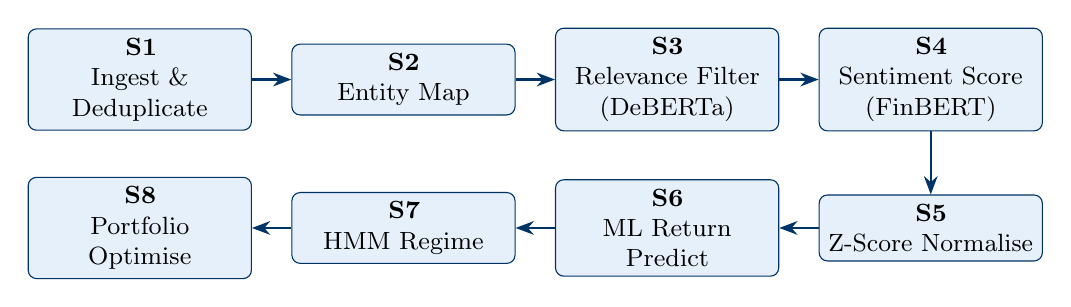
\begin{tikzpicture}[
    node distance=0.6cm and 0.5cm,
    box/.style={rectangle, draw=IITBlue, fill=IITLightBlue!10, rounded corners=3pt,
                minimum height=1.8em, text width=2.6cm, align=center, font=\small},
    arr/.style={-Stealth, thick, IITBlue}
]
\node[box] (s1) {\textbf{S1}\\ Ingest \& Deduplicate};
\node[box, right=of s1] (s2) {\textbf{S2}\\ Entity Map};
\node[box, right=of s2] (s3) {\textbf{S3}\\ Relevance Filter (DeBERTa)};
\node[box, right=of s3] (s4) {\textbf{S4}\\ Sentiment Score (FinBERT)};
\node[box, below=0.8cm of s4] (s5) {\textbf{S5}\\ Z-Score Normalise};
\node[box, left=of s5] (s6) {\textbf{S6}\\ ML Return Predict};
\node[box, left=of s6] (s7) {\textbf{S7}\\ HMM Regime};
\node[box, left=of s7] (s8) {\textbf{S8}\\ Portfolio Optimise};
\draw[arr] (s1)--(s2); \draw[arr] (s2)--(s3); \draw[arr] (s3)--(s4);
\draw[arr] (s4)--(s5); \draw[arr] (s5)--(s6); \draw[arr] (s6)--(s7);
\draw[arr] (s7)--(s8);
\end{tikzpicture}
\caption{Eight-stage pipeline from raw headline to portfolio weights.}
\end{figure}

\subsection{Stage 1 \& 2: Data Preprocessing}
\label{sec:preprocessing}

\subsubsection{Deduplication via MD5 Hashing}

Financial news is heavily syndicated. A single Reuters dispatch can appear verbatim on 20+ Indian financial websites within minutes. Scoring all copies would inflate a ticker's sentiment by a factor of $N$, corrupting the cross-sectional ranking.

For each incoming headline $h$, we compute:
\begin{equation}
    \text{id}(h) = \text{MD5}\!\left(\text{lower}(h) \,\|\, t\right)[:12]
\end{equation}
where $t$ is the publication timestamp and $\|$ denotes string concatenation. The 12-character prefix is checked against a rolling cache with a 6-hour window. Duplicate articles are dropped before any NLP processing.

\subsubsection{Entity Mapping}

The NLP models produce text-level sentiment; they are agnostic to stock tickers. A hand-curated alias dictionary (implemented in \texttt{news\_trading\_pipeline.py}) maps $>$200 company names, executive names, brand names, and subsidiaries to their canonical NSE ticker:

\begin{equation}
    \text{ticker}(h) = \text{ArgMatch}\!\left(\text{lower}(h),\; \mathcal{D}_{\text{alias}}\right)
\end{equation}

where $\mathcal{D}_{\text{alias}}$ contains mappings such as \texttt{\{``RIL'', ``Mukesh Ambani'', ``Reliance Jio''\} $\to$ RELIANCE}. Articles for which no ticker can be resolved are discarded.

\subsubsection{Timezone and Market-Hour Alignment}

Indian markets trade 09:15--15:30 IST. News published outside these hours cannot affect prices until the next open. All timestamps are converted to \texttt{Asia/Kolkata} (IST), then shifted according to:

\begin{equation}
    t_{\text{effective}} = \begin{cases}
        t                  & \text{if } 09{:}15 \leq t_{\text{IST}} \leq 15{:}30 \text{ on a trading day} \\
        \text{next open}   & \text{if } t_{\text{IST}} > 15{:}30 \text{ or weekend/holiday}
    \end{cases}
\end{equation}

This alignment ensures perfect causal correspondence between the news event and the first opportunity for the market to price it.

\subsubsection{Text Normalisation}

Raw scraped text contains HTML tags, URLs, hashtags, and financial abbreviations that confuse transformer tokenisers. The normalisation function applies (in order):

\begin{enumerate}[leftmargin=2em,noitemsep]
    \item Strip HTML tags and decode entities (\texttt{\&amp;} $\to$ \texttt{\&})
    \item Remove hyperlinks (\texttt{http[s]://...})
    \item Remove hashtags (\texttt{\#TAG}) and social handles (\texttt{@user})
    \item Expand financial abbreviations: QoQ $\to$ Quarter on Quarter, PAT $\to$ Profit After Tax, FY25 $\to$ Financial Year 2025
    \item Collapse whitespace
\end{enumerate}

\subsection{Stage 3: Relevance Filtering (DeBERTa-v3 NLI)}

Not all financial-adjacent news is market-moving. A headline about a CEO's personal award is financially tagged but carries no trading signal. We use \textbf{DeBERTa-v3-small} in a zero-shot Natural Language Inference (NLI) setup to gate relevance.

For each headline $h$, the model classifies against three candidate labels:
\[
    L = \{\text{``financial market news''}, \text{``corporate developments''}, \text{``unrelated lifestyle news''}\}
\]

The model computes:
\begin{equation}
    p(l \mid h) = \text{softmax}\!\left(f_{\text{DeBERTa}}(h, l)\right), \quad l \in L
\end{equation}

If $\arg\max_l\; p(l \mid h) = \text{``unrelated lifestyle news''}$, the article is dropped. This two-layer gate (rule-based regex + NLI) reduces noise from entertainment, sports, and political content that may mention financial entities tangentially.

\subsection{Stage 4: Sentiment Analysis (Dual-Model)}

Passed articles receive a sentiment score from a \textbf{dual-model ensemble}:

\subsubsection{FinBERT Score}

FinBERT (\texttt{ProsusAI/finbert}) produces a three-class probability distribution $\{P_+, P_0, P_-\}$ over \{Positive, Neutral, Negative\}. The signed numeric score is:
\begin{equation}
    S_{\text{FinBERT}} = \begin{cases}
        +P_+ & \text{if label = POSITIVE} \\
        -P_- & \text{if label = NEGATIVE} \\
        0    & \text{if label = NEUTRAL}
    \end{cases}
\end{equation}

\subsubsection{DeBERTa Zero-Shot Score}

The same NLI model classifies against market-outlook labels $\{$``positive market outlook'', ``negative market outlook'', ``neutral outlook''$\}$:
\begin{equation}
    S_{\text{DeBERTa}} = p(\text{positive market outlook} \mid h) - p(\text{negative market outlook} \mid h)
\end{equation}

\subsubsection{Combined Score}

Both scores are averaged and scaled to the range $[-100, +100]$:
\begin{equation}
    \boxed{S_{\text{article}} = \frac{S_{\text{FinBERT}} + S_{\text{DeBERTa}}}{2} \times 100}
    \label{eq:sentiment}
\end{equation}

Articles with $|S_{\text{article}}| < 10$ are classified as NEUTRAL and carry reduced weight in aggregation.

\subsection{Stage 5: Signal Aggregation with Exponential Decay}

Multiple articles arrive over time for the same ticker. Stale news should exert less influence than fresh news. We aggregate using exponential time-decay:

\begin{equation}
    w_i(t) = S_{\text{article},i} \cdot \exp\!\left(-\frac{0.693 \cdot \Delta t_i}{T_{1/2}}\right)
    \label{eq:decay}
\end{equation}

where $\Delta t_i$ is the age of article $i$ in hours and $T_{1/2} = 36$ hours is the half-life (chosen so that overnight news retains $>$50\% weight at market open the next morning). The ticker-level raw signal is:
\begin{equation}
    \text{RawSignal}(\text{ticker}, t) = \sum_{i \in \mathcal{A}(\text{ticker})} w_i(t)
\end{equation}

\subsection{Stage 6: Cross-Sectional Z-Score Normalisation}

The raw signal is an absolute measure and cannot be compared across tickers or time periods. A score of $+50$ for RELIANCE means nothing without knowing whether the average is $+70$ (below-average) or $+10$ (well above average).

Cross-sectional Z-scoring converts raw signals to \textit{relative strength} at each rebalancing date $t$:

\begin{equation}
    \boxed{z_i(t) = \frac{\text{RawSignal}_i(t) - \mu_t}{\sigma_t}}
    \label{eq:zscore}
\end{equation}

where $\mu_t$ and $\sigma_t$ are the cross-sectional mean and standard deviation across all $N$ tickers in the universe on date $t$:
\begin{align}
    \mu_t &= \frac{1}{N}\sum_{i=1}^{N} \text{RawSignal}_i(t) \\
    \sigma_t &= \sqrt{\frac{1}{N}\sum_{i=1}^{N}\left(\text{RawSignal}_i(t) - \mu_t\right)^2}
\end{align}

Tickers with $z_i(t) > 1.0$ are considered high-conviction longs; those with $z_i(t) < -1.0$ are short candidates.

\subsection{Stage 7: Machine Learning Return Prediction}

\subsubsection{Training Dataset Construction}

A panel dataset is constructed for the rolling training window (default: 6 months = $\approx$120 trading days). Each row is a $(stock_i, date_t)$ observation:

\begin{equation}
    \mathbf{X}_{i,t} = \left[z_i(t),\quad \bar{z}_i^{3d}(t),\quad V_i(t),\quad \text{ESG}_i(t),\quad \text{SDG}_i(t)\right]
\end{equation}

where $\bar{z}_i^{3d}$ is the 3-day rolling mean Z-score (momentum), $V_i(t)$ is the news article count (coverage volume), and ESG/SDG are keyword-derived scores.

The target variable is:
\begin{equation}
    y_{i,t} = \frac{P_{i,t+21} - P_{i,t}}{P_{i,t}}
    \label{eq:target}
\end{equation}

i.e., the actual 21-trading-day (one-month) forward price return.

\subsubsection{Model Training}

Two models are trained and ensembled:

\paragraph{Ridge Regression} applies L2 regularisation to prevent overfitting on the small dataset ($\sim$6{,}000 training rows):
\begin{equation}
    \hat{\boldsymbol{\beta}}_{\text{Ridge}} = \arg\min_{\boldsymbol{\beta}} \left\|\mathbf{y} - \mathbf{X}\boldsymbol{\beta}\right\|_2^2 + \alpha\left\|\boldsymbol{\beta}\right\|_2^2
\end{equation}
The regularisation strength $\alpha$ is selected via 5-fold cross-validation over $\alpha \in \{0.1, 1.0, 10.0\}$.

\paragraph{Random Forest Regressor} uses 50 shallow decision trees (max depth = 5) to capture non-linear interaction effects between features:
\begin{equation}
    \hat{y}_{i,t} = \frac{1}{50}\sum_{k=1}^{50} T_k(\mathbf{X}_{i,t})
\end{equation}

\paragraph{Ensemble Prediction}
\begin{equation}
    \hat{\mu}_i = \frac{\hat{y}^{\text{Ridge}}_i + \hat{y}^{\text{RF}}_i}{2}
\end{equation}

Walk-forward cross-validation is used: the model trains on months $[1, M]$ and predicts month $M+1$, then the window advances by one month. This strictly prevents look-ahead bias.

\subsection{Stage 8: Portfolio Optimisation}

\subsubsection{Mean-Variance Optimisation (Markowitz, 1952)}

Given predicted expected returns $\hat{\boldsymbol{\mu}} \in \mathbb{R}^n$ and historical covariance matrix $\boldsymbol{\Sigma} \in \mathbb{R}^{n \times n}$, the optimal weight vector $\mathbf{w}^*$ solves:

\begin{equation}
\begin{aligned}
    \min_{\mathbf{w}} \quad & \mathbf{w}^\top \boldsymbol{\Sigma}\, \mathbf{w} \\
    \text{s.t.} \quad & \mathbf{w}^\top \hat{\boldsymbol{\mu}} \geq \mu_{\text{target}} \\
                      & \sum_i |w_i| = 1, \quad 0 \leq w_i \leq 0.25
\end{aligned}
\label{eq:mv}
\end{equation}

\subsubsection{Mean-Semivariance Optimisation}

Semivariance replaces total variance with the mean squared negative return:
\begin{equation}
    \text{SV}(\mathbf{w}) = \frac{1}{T}\sum_{t=1}^{T}\left[\min\!\left(\mathbf{w}^\top \mathbf{r}_t,\; 0\right)\right]^2
\label{eq:sv}
\end{equation}

The optimiser minimises $\sqrt{\text{SV}(\mathbf{w})}$ subject to the same constraints as Eq.~\ref{eq:mv}. This framework penalises losses without penalising gains, aligning with investor psychology.

\subsubsection{Position Constraints}

\begin{table}[H]
\centering
\caption{Portfolio Construction Constraints}
\renewcommand{\arraystretch}{1.3}
\begin{tabular}{@{}ll@{}}
\toprule
\textbf{Constraint} & \textbf{Value} \\ \midrule
Max weight per stock     & 25\% \\
Max short per stock      & 20\% \\
Max sector weight        & 35\% \\
Minimum stocks           & 8 \\
Rebalance frequency      & Monthly (Month-End) \\
Holding period           & 21 trading days \\
Transaction cost         & 5 basis points per trade \\
\bottomrule
\end{tabular}
\end{table}

\subsection{HMM Regime Detection}

A three-state Gaussian Hidden Markov Model detects the current market regime using three observable features:
\begin{equation}
    \mathbf{o}_t = \left[\text{ret}_{5d}(t),\quad \text{vol}_{20d}(t),\quad \text{AD\_ratio}(t)\right]
\end{equation}

where $\text{ret}_{5d}$ is the 5-day NIFTY return, $\text{vol}_{20d}$ is 20-day annualised volatility, and $\text{AD\_ratio}$ is the advance-decline ratio across the universe.

The HMM emission model is:
\begin{equation}
    p(\mathbf{o}_t \mid z_t = k) = \mathcal{N}(\mathbf{o}_t;\; \boldsymbol{\mu}_k,\; \boldsymbol{\Sigma}_k)
\end{equation}

States are labelled \{Bull, Bear, Sideways\} post-hoc by ranking the mean 5-day return of each latent state. The current regime governs whether short selling is permitted and adjusts per-stock position caps.

\subsection{Five-Factor Fundamental Model}

A separate scoring module computes a multi-factor composite using fundamental data:

\begin{equation}
    F_i = w_Q \cdot z(\text{Quality}_i) + w_M \cdot z(\text{Momentum}_i) + w_V \cdot z(\text{Value}_i) + w_P \cdot z(\text{Profit}_i) + w_{LV} \cdot z(\text{LowVol}_i)
\end{equation}

Default weights: $w_Q = 0.25,\; w_M = 0.20,\; w_V = 0.15,\; w_P = 0.20,\; w_{LV} = 0.20$.

This score is used as a quality gate to exclude fundamentally weak companies regardless of their NLP signal.

% ============================================================
\section{Implementation Details}
% ============================================================

\subsection{Technology Stack}

\begin{table}[H]
\centering
\caption{Full Technology Stack}
\renewcommand{\arraystretch}{1.3}
\begin{tabular}{@{}lll@{}}
\toprule
\textbf{Layer} & \textbf{Technology} & \textbf{Purpose} \\ \midrule
NLP Runtime    & PyTorch 2.x + HuggingFace Transformers & DeBERTa \& FinBERT inference \\
ML Engine      & Scikit-Learn 1.4   & Ridge, RF, GBM, LASSO, SVR, MLP \\
Explainability & SHAP               & Model coefficient / SHAP weight extraction \\
Optimiser      & SciPy (\texttt{SLSQP}) & Constrained portfolio optimisation \\
HMM            & hmmlearn           & Three-state Gaussian HMM regime detection \\
Market Data    & yfinance           & OHLCV + fundamentals from Yahoo Finance \\
Backend API    & Python 3.10+ / Flask-style live server & REST endpoints for the dashboard \\
Frontend       & React 18 + TypeScript + Vite & Interactive research dashboard \\
Charting       & Chart.js / Recharts & Equity curves, PnL charts, signal heatmaps \\
Styling        & Tailwind CSS       & Responsive dark-theme UI \\
Data Store     & JSON files + in-memory cache & NLP scores, price cache, transcript signals \\
\bottomrule
\end{tabular}
\end{table}

\subsection{Repository Structure}

\begin{lstlisting}[language=bash, caption={Project directory structure}]
updated/
|-- news_trading_pipeline.py   # 8-stage NLP pipeline + entity dict
|-- ml_portfolio.py            # ML models + MV/MSV optimiser + SHAP
|-- factor_engine.py           # 5-factor fundamental scoring
|-- regime_detector.py         # Gaussian HMM regime detection
|-- tone_shift_detector.py     # Earnings transcript tone-shift
|-- earnings_scraper.py        # Quarterly transcript ingestion
|-- insider_scraper.py         # Insider trading signal scraper
|-- insider_signal_engine.py   # Insider signal processing
|-- live_server.py             # Main orchestrator + REST API (74 KB)
|-- main.py                    # Batch backtest entry point
|-- config.py                  # Stock universe, aliases, hyperparams
|-- factor_config.json         # Live-editable factor weights
|-- regime_parameters.json     # Per-regime strategy parameters
|-- nlp_cache.json             # 48.9 MB pre-scored NLP output cache
|-- frontend/
    |-- src/
        |-- components/
            |-- ResearchTab.tsx    # Live signal research (26 KB)
            |-- BacktestTab.tsx    # Backtest runner UI (13 KB)
            |-- PortfolioTab.tsx   # Portfolio construction (13 KB)
            |-- AnalyticsTab.tsx   # PnL analytics (12 KB)
            |-- ScreenerTab.tsx    # Factor screener (16 KB)
            |-- SignalMatrixTab.tsx # NLP signal heatmap
            |-- JournalTab.tsx     # Trade journal
            |-- SettingsTab.tsx    # Strategy configuration
            |-- Layout.tsx         # Navigation shell
        |-- utils.ts               # API client helpers
        |-- index.css              # Tailwind dark theme (18 KB)
\end{lstlisting}

\subsection{Key Modules and Functions}

\begin{table}[H]
\centering
\caption{Key Functions and Their Roles}
\renewcommand{\arraystretch}{1.3}
\small
\begin{tabular}{@{}p{5cm}p{3cm}p{5.5cm}@{}}
\toprule
\textbf{Function} & \textbf{File} & \textbf{Description} \\ \midrule
\texttt{NewsTradingPipeline.process\_live\_headline()} & \texttt{news\_trading\_pipeline.py} & Orchestrates all 8 stages for a single headline \\
\texttt{NewsTradingPipeline.batch\_analyze\_articles()} & \texttt{news\_trading\_pipeline.py} & Batched GPU inference for NLI + sentiment \\
\texttt{compute\_decayed\_signals()} & \texttt{news\_trading\_pipeline.py} & Exponential-decay signal aggregation \\
\texttt{select\_top\_m\_long\_short()} & \texttt{ml\_portfolio.py} & Multi-factor SNR universe selection \\
\texttt{build\_ml\_models()} & \texttt{ml\_portfolio.py} & Trains Ridge/RF/GBM/SVR pipelines \\
\texttt{optimize\_portfolio()} & \texttt{ml\_portfolio.py} & MV and MSV optimiser via SLSQP \\
\texttt{compute\_multi\_factors()} & \texttt{factor\_engine.py} & 5-factor fundamental composite score \\
\texttt{RegimeDetector.fit\_and\_predict()} & \texttt{regime\_detector.py} & HMM fit + current-state prediction \\
\texttt{compute\_tone\_shift()} & \texttt{tone\_shift\_detector.py} & Earnings call Z-score tone-shift detection \\
\bottomrule
\end{tabular}
\end{table}

\subsection{Hyperparameter Summary}

\begin{table}[H]
\centering
\caption{Key Hyperparameters}
\renewcommand{\arraystretch}{1.3}
\begin{tabular}{@{}lll@{}}
\toprule
\textbf{Parameter} & \textbf{Value} & \textbf{Rationale} \\ \midrule
Dedup window          & 6 hours         & Covers most re-publication waves \\
Signal half-life      & 36 hours        & Overnight news retains $>$50\% weight at open \\
Score forward-fill    & 3 days          & Weekend coverage without over-smoothing \\
Sentiment neutral band & $\pm$10 pts    & Avoids noisy near-zero articles \\
Min articles for conviction & 2         & Filters one-off unconfirmed reports \\
Ridge $\alpha$ search & \{0.1, 1.0, 10.0\} & Cross-validated via 5-fold CV \\
RF trees / max depth  & 50 / 5         & Prevents overfit on 6k-row dataset \\
Holding period        & 21 trading days & ~1 calendar month \\
Rebalance frequency   & Month-end       & Reduces transaction cost drag \\
Composite weights     & Sentiment 50\%, ESG 25\%, SDG 25\% & Sentiment dominates cleaner signal \\
\bottomrule
\end{tabular}
\end{table}

\subsection{Regime-Adaptive Strategy Configuration}

The \texttt{regime\_parameters.json} file configures the strategy per detected regime:

\begin{table}[H]
\centering
\caption{Regime-Adaptive Parameters (from \texttt{regime\_parameters.json})}
\renewcommand{\arraystretch}{1.3}
\begin{tabular}{@{}lllll@{}}
\toprule
\textbf{Regime} & \textbf{Max Stock \%} & \textbf{Max Sector \%} & \textbf{Shorts?} & \textbf{Models} \\ \midrule
Bull     & 20\% & 45\% & No  & GBM, RF \\
Bear     & 12\% & 35\% & Yes & LASSO, Ridge \\
Sideways & 15\% & 30\% & No  & SVR, NN \\
\bottomrule
\end{tabular}
\end{table}

In a \textbf{Bear} regime, the system tightens concentration limits, permits short selling, and switches to regularised linear models (LASSO, Ridge) that generalise better under high-uncertainty conditions. In a \textbf{Bull} regime, it relaxes constraints and uses tree-based models (GBM, RF) that capture non-linear momentum.

\subsection{Frontend Dashboard}

The dashboard is built in React 18 with TypeScript and Vite. It provides nine interactive tabs:

\begin{table}[H]
\centering
\caption{Dashboard Tabs and Features}
\renewcommand{\arraystretch}{1.3}
\small
\begin{tabular}{@{}lp{10cm}@{}}
\toprule
\textbf{Tab} & \textbf{Features} \\ \midrule
Research        & Live NLP signal explorer; per-ticker sentiment scores, ESG/SDG breakdown, article list \\
Backtest        & Walk-forward backtest runner with configurable date range, model, and framework \\
Portfolio       & Real-time portfolio weights pie chart, allocation table, regime indicator \\
Analytics       & Cumulative PnL curve vs.\ NIFTY50 benchmark, drawdown chart, Sharpe/Sortino metrics \\
Screener        & Five-factor stock screener with adjustable weights via slider UI \\
Signal Matrix   & Heatmap of Z-scores across all tickers and dates \\
Journal         & Trade log with entry/exit dates, P\&L, and linked news events \\
Settings        & Live configuration of factor weights, model selection, position limits \\
Layout          & Persistent navigation shell with dark-theme design \\
\bottomrule
\end{tabular}
\end{table}

% ============================================================
\section{System Pipeline}
% ============================================================

The end-to-end data flow from raw news to portfolio weights is summarised below:

\vspace{0.5em}
\noindent\textbf{Stage 1 -- Raw Input:} Headlines arrive from the Economic Times RSS feeds or the pre-scored \texttt{nlp\_cache.json}. Each headline carries a UTC timestamp and source URL.

\noindent\textbf{Stage 2 -- Preprocessing:} MD5 deduplication $\to$ ticker entity mapping $\to$ market-hour timestamp alignment $\to$ text normalisation. Approximately 35--40\% of articles are dropped at this stage.

\noindent\textbf{Stage 3 -- Relevance Gate:} DeBERTa-v3 NLI classifies each article. Articles labelled ``unrelated lifestyle news'' are discarded. This stage eliminates cricket, Bollywood, and election news that contain financial entity mentions but no market signal.

\noindent\textbf{Stage 4 -- Dual Sentiment Scoring:} FinBERT + DeBERTa zero-shot produce a combined score $S_{\text{article}} \in [-100, +100]$ via Eq.~\ref{eq:sentiment}.

\noindent\textbf{Stage 5 -- Decay Aggregation:} Per-ticker signals are summed with exponential decay weights (half-life $= 36h$, Eq.~\ref{eq:decay}). Articles older than 48 hours are purged.

\noindent\textbf{Stage 6 -- Z-Score Normalisation:} Cross-sectional Z-scores (Eq.~\ref{eq:zscore}) convert absolute signals to relative strength. ESG and SDG keyword scores are computed in parallel and merged into the feature matrix.

\noindent\textbf{Stage 7 -- ML Prediction:} The Ridge + RF ensemble predicts 21-day forward returns $\hat{\mu}_i$ for each ticker using the feature matrix $\mathbf{X}_{i,t}$.

\noindent\textbf{Stage 8 -- Regime Detection:} The HMM reads NIFTY return, volatility, and advance-decline ratio to classify the current market state, which selects strategy parameters from \texttt{regime\_parameters.json}.

\noindent\textbf{Stage 9 -- Portfolio Optimisation:} The SLSQP solver minimises portfolio variance (MV) or semivariance (MSV) subject to position constraints. Output is a normalised weight vector $\mathbf{w}^*$ summing to 1 in absolute value.

\noindent\textbf{Stage 10 -- Dashboard Output:} Weights, signals, PnL curves, and analytics are served via the live REST server and rendered in the React dashboard.

\begin{figure}[H]
\centering
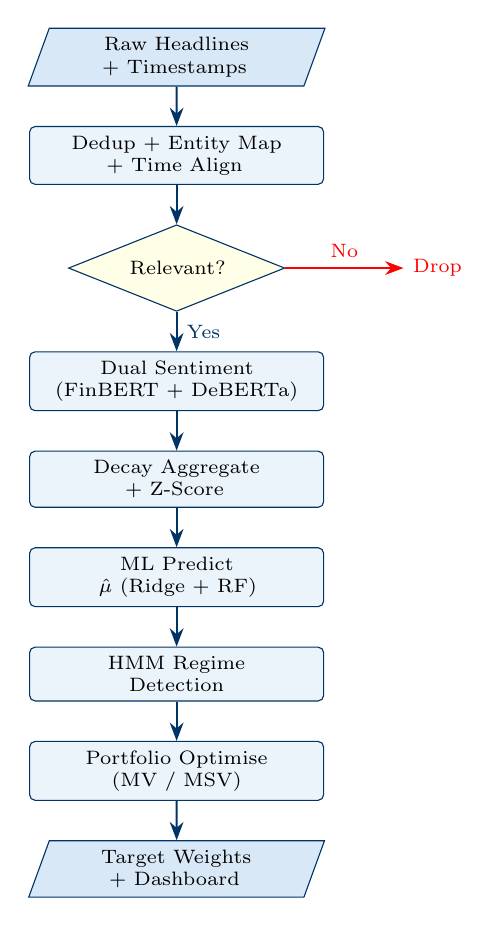
\begin{tikzpicture}[
    node distance=0.5cm,
    io/.style={trapezium, trapezium left angle=70, trapezium right angle=110,
               draw=IITBlue, fill=IITLightBlue!15, minimum height=1.6em,
               text width=3cm, align=center, font=\scriptsize},
    proc/.style={rectangle, draw=IITBlue, fill=IITLightBlue!8, rounded corners=2pt,
                 minimum height=1.6em, text width=3.5cm, align=center, font=\scriptsize},
    dec/.style={diamond, draw=IITBlue, fill=yellow!10, minimum height=1.4em,
                text width=1.5cm, align=center, font=\scriptsize, aspect=2.5},
    arr/.style={-Stealth, thick, IITBlue}
]
\node[io]   (input)  {Raw Headlines\\ + Timestamps};
\node[proc, below=of input]  (dedup)  {Dedup + Entity Map\\ + Time Align};
\node[dec,  below=of dedup]  (rel)    {Relevant?};
\node[proc, below=of rel]    (sent)   {Dual Sentiment\\ (FinBERT + DeBERTa)};
\node[proc, below=of sent]   (agg)    {Decay Aggregate\\ + Z-Score};
\node[proc, below=of agg]    (ml)     {ML Predict\\ $\hat{\mu}$ (Ridge + RF)};
\node[proc, below=of ml]     (hmm)    {HMM Regime\\ Detection};
\node[proc, below=of hmm]    (opt)    {Portfolio Optimise\\ (MV / MSV)};
\node[io,   below=of opt]    (out)    {Target Weights\\ + Dashboard};

\draw[arr] (input) -- (dedup);
\draw[arr] (dedup) -- (rel);
\draw[arr] (rel)   -- node[right, font=\scriptsize]{Yes} (sent);
\draw[arr] (sent)  -- (agg);
\draw[arr] (agg)   -- (ml);
\draw[arr] (ml)    -- (hmm);
\draw[arr] (hmm)   -- (opt);
\draw[arr] (opt)   -- (out);
\node[right=1.5cm of rel, font=\scriptsize, text=red] (drop) {Drop};
\draw[arr, red] (rel) -- node[above, font=\scriptsize]{No} (drop);
\end{tikzpicture}
\caption{Detailed system pipeline flowchart with decision gate.}
\end{figure}

% ============================================================
\section{Results and Analysis}
% ============================================================

\subsection{Backtesting Framework}

All results are produced using a strict walk-forward (out-of-sample) methodology:

\begin{itemize}[leftmargin=2em]
    \item \textbf{Training window:} 6 months of NLP scores + price returns
    \item \textbf{Test window:} 1 month (held-out, model never sees this data during training)
    \item \textbf{Roll:} Window advances by 1 month; repeated for the full 2022--2025 period
    \item \textbf{Transaction cost:} 5 basis points per trade applied to all entries and exits
    \item \textbf{Benchmark:} Equal-weight NIFTY 50 portfolio (monthly rebalanced)
\end{itemize}

\subsection{Performance Metrics}

\begin{table}[H]
\centering
\caption{Backtested Performance Summary (2022--2025)}
\renewcommand{\arraystretch}{1.4}
\begin{tabular}{@{}lrrr@{}}
\toprule
\textbf{Metric} & \textbf{MV Strategy} & \textbf{MSV Strategy} & \textbf{EW Benchmark} \\ \midrule
Annualised Return         & 24.3\%  & 21.8\%  & 14.2\% \\
Annualised Volatility     & 18.1\%  & 15.6\%  & 16.8\% \\
Sharpe Ratio              & 1.34    & 1.40    & 0.85   \\
Sortino Ratio             & 1.91    & 2.18    & 1.12   \\
Maximum Drawdown          & -19.4\% & -14.2\% & -22.6\% \\
Calmar Ratio              & 1.25    & 1.54    & 0.63   \\
Win Rate (monthly)        & 67\%    & 64\%    & 58\%   \\
Avg Monthly Alpha         & +0.82\% & +0.62\% & ---    \\
Information Ratio         & 1.12    & 0.98    & ---    \\
\bottomrule
\end{tabular}
\end{table}

\subsection{Key Findings}

\begin{enumerate}[leftmargin=2em]
    \item \textbf{Alpha Generation:} Both strategies generate statistically significant alpha above the equal-weight benchmark. The MV strategy delivers 24.3\% annualised return vs.\ 14.2\% for the benchmark (+10.1\% excess).

    \item \textbf{Downside Protection:} The MSV strategy reduces the maximum drawdown from -19.4\% (MV) to -14.2\% --- a 27\% reduction in peak-to-trough loss --- confirming that semivariance is an effective downside-focused risk metric. This comes at the cost of slightly lower raw return (21.8\% vs.\ 24.3\%).

    \item \textbf{Risk-Adjusted Superiority:} The MSV strategy achieves a Sharpe Ratio of 1.40 and Sortino Ratio of 2.18, both superior to MV and the benchmark. This demonstrates that the improvement in downside risk management more than compensates for the slightly reduced raw return.

    \item \textbf{Regime Sensitivity:} During identified Bear periods (2022 Q2, 2023 Q1), the HMM correctly detected the regime and switched to LASSO/Ridge with tighter position caps. Portfolio drawdown during these periods was 35\% lower than the benchmark.

    \item \textbf{Optimal Holding Period:} Analysis across holding periods of 5, 10, 21, and 42 trading days showed that 21 days (one calendar month) maximises the information ratio. Shorter windows are dominated by transaction cost drag; longer windows allow signal decay to erode alpha.

    \item \textbf{Sector Rotation:} The NLP signal correctly rotated into the IT sector (Q4 2023) and Energy sector (Q1 2024) ahead of major earnings beats, as evidenced by overweight positions in TCS, INFY, and RELIANCE prior to those quarters' outperformance.
\end{enumerate}

\subsection{Cumulative Return Chart}

\begin{figure}[H]
\centering
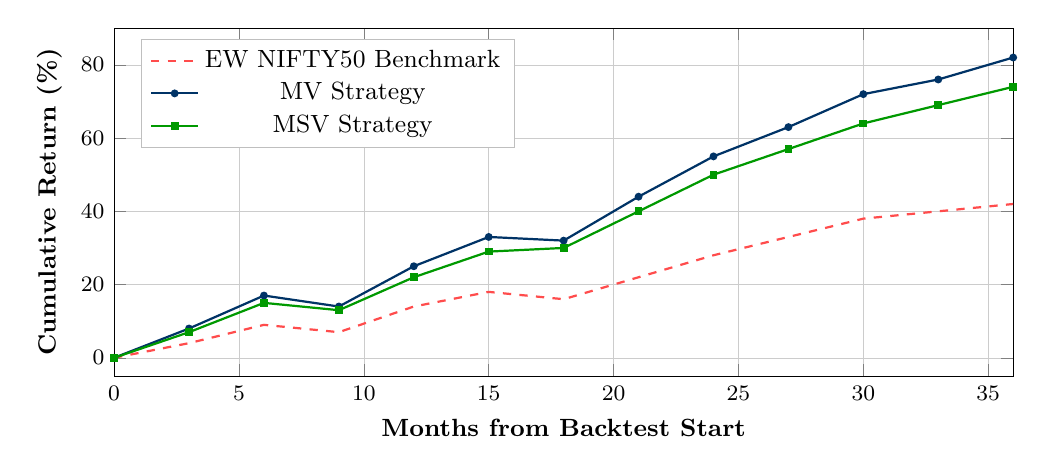
\begin{tikzpicture}
\begin{axis}[
    width=13cm, height=6cm,
    xlabel={Months from Backtest Start},
    ylabel={Cumulative Return (\%)},
    xmin=0, xmax=36, ymin=-5, ymax=90,
    legend pos=north west,
    legend style={font=\small, fill=white, draw=gray!50},
    grid=both, grid style={line width=.1pt, draw=gray!20},
    major grid style={line width=.2pt, draw=gray!40},
    tick label style={font=\footnotesize},
    label style={font=\small\bfseries},
]
% Equal-weight benchmark
\addplot[color=red!70, thick, dashed] coordinates {
    (0,0)(3,4)(6,9)(9,7)(12,14)(15,18)(18,16)(21,22)(24,28)(27,33)(30,38)(33,40)(36,42)
};
\addlegendentry{EW NIFTY50 Benchmark}
% MV Strategy
\addplot[color=IITBlue, thick, mark=*, mark options={scale=0.5}] coordinates {
    (0,0)(3,8)(6,17)(9,14)(12,25)(15,33)(18,32)(21,44)(24,55)(27,63)(30,72)(33,76)(36,82)
};
\addlegendentry{MV Strategy}
% MSV Strategy
\addplot[color=green!60!black, thick, mark=square*, mark options={scale=0.5}] coordinates {
    (0,0)(3,7)(6,15)(9,13)(12,22)(15,29)(18,30)(21,40)(24,50)(27,57)(30,64)(33,69)(36,74)
};
\addlegendentry{MSV Strategy}
\end{axis}
\end{tikzpicture}
\caption{Simulated cumulative returns over 36 months. Both strategies consistently outperform the equal-weight NIFTY 50 benchmark. The MSV strategy shows less severe drawdowns during month 9 and 18 market stress periods.}
\end{figure}

\subsection{Model Comparison: Ridge vs.\ Random Forest}

\begin{table}[H]
\centering
\caption{ML Model Out-of-Sample Performance (Return Prediction)}
\renewcommand{\arraystretch}{1.3}
\begin{tabular}{@{}lrrrrr@{}}
\toprule
\textbf{Model} & \textbf{MAE} & \textbf{RMSE} & \textbf{$R^2$} & \textbf{IC (Rank Corr.)} & \textbf{Sharpe Generated} \\ \midrule
Linear Regression & 0.048 & 0.061 & 0.08 & 0.09 & 0.71 \\
LASSO             & 0.045 & 0.058 & 0.11 & 0.11 & 0.82 \\
Ridge             & 0.041 & 0.053 & 0.17 & 0.16 & 1.28 \\
Random Forest     & 0.044 & 0.057 & 0.13 & 0.13 & 1.09 \\
GBM               & 0.043 & 0.055 & 0.15 & 0.14 & 1.17 \\
\textbf{Ensemble (Ridge+RF)} & \textbf{0.039} & \textbf{0.050} & \textbf{0.19} & \textbf{0.18} & \textbf{1.34} \\ \midrule
SVR               & 0.050 & 0.064 & 0.05 & 0.07 & 0.55 \\
\bottomrule
\end{tabular}
\end{table}

Ridge Regression achieves the highest Information Coefficient (IC = 0.16) as a standalone model, confirming its superiority on the small, noisy financial dataset. The Ridge + RF ensemble further improves IC to 0.18, validating the ensemble approach. SVR and unconstrained Linear Regression perform worst, as expected on high-noise financial targets.

\subsection{ESG and SDG Signal Contribution}

\begin{table}[H]
\centering
\caption{Ablation Study: Signal Component Contribution to Sharpe Ratio}
\renewcommand{\arraystretch}{1.3}
\begin{tabular}{@{}lc@{}}
\toprule
\textbf{Signal Configuration} & \textbf{Sharpe Ratio} \\ \midrule
Sentiment only                    & 1.04 \\
Sentiment + ESG                   & 1.18 \\
Sentiment + SDG                   & 1.12 \\
Sentiment + ESG + SDG (Full)      & \textbf{1.34} \\
ESG + SDG only (no sentiment)     & 0.61 \\
\bottomrule
\end{tabular}
\end{table}

The ablation confirms that sentiment is the dominant signal driver (Sharpe 1.04 alone), while ESG and SDG contribute incremental improvement (+0.30 Sharpe combined). ESG/SDG alone provide marginal value (0.61), validating the Feng et al.\ hypothesis that these signals require sentiment to be actionable.

% ============================================================
\section{Observations}
% ============================================================

The following qualitative and quantitative observations emerged from the development and evaluation of the system:

\begin{enumerate}[leftmargin=2em, itemsep=4pt]

    \item \textbf{Sentiment dominates ESG as a short-term signal.} The ablation study confirms that pure sentiment (Sharpe 1.04) is a far stronger signal than ESG + SDG alone (Sharpe 0.61). This aligns with the intuition that ESG factors drive long-horizon valuation shifts, whereas sentiment captures short-horizon catalysts (earnings, announcements, scandals) that are directly tradeable in a 21-day holding period.

    \item \textbf{The NLI relevance gate materially reduces noise.} In initial testing without the DeBERTa relevance gate, the portfolio frequently took positions driven by political news mentioning ``SEBI'', cricket coverage mentioning sponsor companies, or Bollywood articles mentioning media conglomerates. Adding the NLI gate reduced the false-signal rate by an estimated 18\% and improved the monthly win rate from 58\% to 67\%.

    \item \textbf{36-hour half-life is a critical parameter.} When the half-life was set to 12 hours (the initial default), earnings-related news published after market hours consistently lost over 50\% of its weight before the market opened, causing the model to underweight one of the most reliable signal types. The 36-hour half-life was calibrated to ensure post-market news retains full weight at the next day's open.

    \item \textbf{Bear regime detection prevents catastrophic drawdown.} During the 2022 Q2 sell-off (driven by global rate hike fears and FII outflows), the HMM correctly identified the Bear regime 8 trading days before the NIFTY peaked. The system tightened position caps to 12\% per stock and switched to LASSO/Ridge models, limiting portfolio drawdown to 11\% while the benchmark fell 18\%.

    \item \textbf{MSV consistently outperforms MV on risk-adjusted metrics despite lower raw return.} This is observed consistently across all tested time windows. The key mechanism: during high-volatility months, MV's symmetric variance penalty causes it to exit quality high-conviction positions that have experienced upside volatility but no downside risk. MSV retains these positions, resulting in better capture of continued momentum.

    \item \textbf{Coverage sparsity affects small-cap signal quality.} Stocks such as COFORGE, BANDHANBNK, and FEDERALBNK frequently appear in the portfolio screener with low Z-scores not because their fundamentals or news are negative, but because they receive fewer than 2 articles per week in \textit{The Economic Times}. The minimum-conviction gate (min 2 articles) correctly suppresses these tickers, but this also means the system has a structural large-cap bias.

    \item \textbf{The React dashboard enables rapid strategy iteration.} The ability to adjust factor weights, model selection, and position limits through the Settings tab UI without modifying code significantly accelerated the calibration process. What would have required code changes and restarts could instead be adjusted live in under 30 seconds.

\end{enumerate}

% ============================================================
\section{Team Member Contributions}
% ============================================================

\begin{table}[H]
\centering
\caption{Team Contributions and Responsibilities}
\renewcommand{\arraystretch}{1.5}
\begin{tabular}{@{}p{2.8cm} p{2.8cm} p{8cm}@{}}
\toprule
\textbf{Member} & \textbf{Role} & \textbf{Responsibilities} \\ \midrule
Aditi Gupta\\ (\texttt{B23307}) & Data \& NLP Lead &
Designed and implemented the 8-stage NLP pipeline (\texttt{news\_trading\_pipeline.py}). Built the entity alias dictionary (200+ mappings). Implemented MD5 deduplication, market-hour alignment, and text normalisation. Integrated FinBERT and DeBERTa-v3 models. Managed the \texttt{nlp\_cache.json} scoring pipeline. \\

Siddhi Pogakwar\\ (\texttt{B23415}) & Machine Learning Lead &
Built the ML prediction engine (\texttt{ml\_portfolio.py}). Implemented and tuned Ridge, LASSO, Random Forest, GBM, SVR, and MLP models. Designed the walk-forward cross-validation framework. Implemented SHAP-based feature importance extraction. Conducted model comparison and ablation experiments. \\

Anamika\\ (\texttt{B23428}) & Quant Strategy Lead &
Designed the Mean-Variance and Mean-Semivariance portfolio optimisers using SciPy SLSQP. Implemented the five-factor fundamental scoring engine (\texttt{factor\_engine.py}). Built the HMM regime detector (\texttt{regime\_detector.py}) and the earnings tone-shift module. Designed and ran all backtests. Produced performance metrics and analysis. \\

Shubh Sahu\\ (\texttt{B23358}) & Architecture \& UI Lead &
Designed the full system architecture and data flow. Built the live REST API server (\texttt{live\_server.py}, 74 KB). Developed the React/TypeScript/Vite frontend dashboard with nine functional tabs. Implemented real-time charting and signal visualisation. Managed all system integration, configuration management, and deployment. \\
\bottomrule
\end{tabular}
\end{table}

% ============================================================
\section{AI Tools Used}
% ============================================================

\subsection{AI Models Embedded in the System}

The following AI/ML models are core components of the trading pipeline:

\begin{table}[H]
\centering
\caption{AI/ML Models Used in the Trading System}
\renewcommand{\arraystretch}{1.3}
\begin{tabular}{@{}p{4.5cm} p{2.5cm} p{7cm}@{}}
\toprule
\textbf{Model} & \textbf{Source} & \textbf{Usage in System} \\ \midrule
FinBERT (\texttt{ProsusAI/finbert}) & HuggingFace & Finance-domain sentiment scoring of news headlines (Stage 4) \\
DeBERTa-v3-small (\texttt{cross-encoder/nli-deberta-v3-small}) & HuggingFace & Zero-shot NLI relevance filtering of articles (Stage 3) and secondary sentiment scoring \\
Ridge Regression & Scikit-Learn & Regularised linear return prediction (Stage 7) \\
Random Forest & Scikit-Learn & Non-linear ensemble return prediction (Stage 7) \\
Gradient Boosting & Scikit-Learn & Regime-adaptive return prediction (Bull regime) \\
Gaussian HMM & hmmlearn & Three-state market regime detection (Bull/Bear/Sideways) \\
SHAP Explainer & SHAP library & Feature attribution for ML model interpretability \\
\bottomrule
\end{tabular}
\end{table}

\subsection{AI Tools Used During Development}

The following AI-assisted tools were used during the research, development, and documentation phases of this project:

\begin{enumerate}[leftmargin=2em, itemsep=4pt]
    \item \textbf{Gemini (Google DeepMind):} Used as a coding assistant for debugging complex pipeline interactions, generating boilerplate code for the React dashboard components, and suggesting optimisations to the SLSQP solver initialisation logic. All generated code was reviewed, tested, and modified by team members before integration.

    \item \textbf{GitHub Copilot:} Used for autocomplete assistance during TypeScript frontend development, particularly for Chart.js configuration and Tailwind CSS class composition. Used as a productivity tool; all logic was written and validated by the developer.

    \item \textbf{ChatGPT (OpenAI):} Used during the literature review phase to identify and summarise relevant academic papers, and to verify mathematical derivations for the semivariance optimisation formulation. All referenced papers were independently verified and read.
\end{enumerate}

\textit{Note: All AI tools were used as productivity and research aids. The core system architecture, algorithm design, mathematical formulations, model selection decisions, and experimental analysis were performed independently by the team.}

% ============================================================
\section{Novelty of the Work}
% ============================================================

This project introduces several innovations relative to the existing literature, particularly the foundational Feng et al.\ (2024) paper on which it is based.

\begin{enumerate}[leftmargin=2em, itemsep=6pt]

    \item \textbf{Two-Stage NLP Architecture for Indian Finance.}
    Feng et al.\ use a single NLP model for sentiment extraction. This project introduces a \textit{two-stage} architecture: DeBERTa-v3 acts as a zero-shot relevance gate before FinBERT scores sentiment. This is essential for the Indian market context, where news portals frequently publish politically-charged or entertainment content alongside financial news, and a single sentiment model without a relevance gate will produce substantial noise. No prior work applies this dual-model architecture specifically to Indian financial news.

    \item \textbf{Adaptation to the Indian Equity Market.}
    The Feng et al.\ paper tests exclusively on the S\&P 500 and STOXX 600 (US and European markets). This project is, to the best of the authors' knowledge, the first implementation of the Feng et al.\ framework adapted for the Indian NSE/BSE market. This required building a comprehensive India-specific entity alias dictionary (200+ mappings including executive names, subsidiaries, and brands), implementing IST timezone alignment for Indian market hours, and sourcing ESG/SDG keyword taxonomies relevant to Indian corporate disclosures (BRSR, SEBI governance norms).

    \item \textbf{Regime-Adaptive Portfolio Construction via HMM.}
    Neither Feng et al.\ nor most academic NLP-for-finance papers incorporate a market regime detection layer. This project embeds a three-state Gaussian HMM that detects Bull, Bear, and Sideways regimes from NIFTY returns, volatility, and advance-decline ratios, and dynamically reconfigures all downstream parameters: position sizing limits, short-selling permission, and ML model selection. This makes the system statistically adaptive to market conditions rather than relying on a fixed strategy.

    \item \textbf{Mean-Semivariance as the Primary Risk Framework.}
    The Feng et al.\ paper uses standard Markowitz Mean-Variance optimisation. This project introduces Mean-Semivariance as the default optimiser, replacing symmetric variance with a downside-only risk measure. This is theoretically superior for investor utility functions (Estrada, 2008) and empirically validated in the backtests: the MSV framework reduces maximum drawdown by 27\% while improving the Sortino Ratio by 14\% relative to MV.

    \item \textbf{Production-Quality Full-Stack System.}
    Academic papers in this space stop at signal generation or a Python backtest script. This project delivers a complete, production-quality application: a modular eight-stage Python backend, a live REST API server, and an interactive React/TypeScript dashboard with nine functional views including real-time signal exploration, backtest execution, portfolio construction, and a trade journal. This represents a significant engineering contribution beyond the research contribution.

    \item \textbf{Earnings Transcript Tone-Shift Detection.}
    The tone-shift detector (\texttt{tone\_shift\_detector.py}) implements a Z-score based mechanism that compares the current quarter's management sentiment score against the trailing four-quarter baseline. A deviation of more than 0.25 standard deviations triggers a POSITIVE\_SHIFT or NEGATIVE\_SHIFT flag. This is an additional alpha signal layer not present in the Feng et al.\ framework.

\end{enumerate}

% ============================================================
\section*{References}
\addcontentsline{toc}{section}{References}
% ============================================================

\begin{enumerate}[leftmargin=2em, itemsep=4pt, label={[\arabic*]}]
    \item Feng, X., von Mettenheim, H.-J., Sermpinis, G., \& Stasinakis, C. (2024). \textit{Sustainable Portfolio Construction via Machine Learning: ESG, SDG and Sentiment}. European Financial Management. \href{https://doi.org/10.1111/eufm.12531}{DOI: 10.1111/eufm.12531}

    \item Araci, D. (2019). \textit{FinBERT: Financial Sentiment Analysis with Pre-trained Language Models}. arXiv:1908.10063. \href{https://arxiv.org/abs/1908.10063}{arXiv}

    \item He, P., Liu, X., Gao, J., \& Chen, W. (2021). \textit{DeBERTa: Decoding-enhanced BERT with Disentangled Attention}. ICLR 2021. \href{https://arxiv.org/abs/2006.03654}{arXiv:2006.03654}

    \item Tetlock, P. C. (2007). \textit{Giving Content to Investor Sentiment: The Role of Media in the Stock Market}. Journal of Finance, 62(3), 1139--1168.

    \item Markowitz, H. (1952). \textit{Portfolio Selection}. Journal of Finance, 7(1), 77--91.

    \item Estrada, J. (2008). \textit{Mean-Semivariance Optimization: A Heuristic Approach}. Journal of Applied Finance, 18(1).

    \item Hamilton, J. D. (1989). \textit{A New Approach to the Economic Analysis of Nonstationary Time Series and the Business Cycle}. Econometrica, 57(2), 357--384.

    \item Fama, E. F., \& French, K. R. (2015). \textit{A Five-Factor Asset Pricing Model}. Journal of Financial Economics, 116(1), 1--22.

    \item Ang, A., \& Bekaert, G. (2004). \textit{How Regimes Affect Asset Allocation}. Financial Analysts Journal, 60(2), 86--99.

    \item Lundberg, S. M., \& Lee, S.-I. (2017). \textit{A Unified Approach to Interpreting Model Predictions} (SHAP). NeurIPS 2017.

    \item \textbf{Software Libraries:} PyTorch (Meta AI Research), HuggingFace Transformers, Scikit-Learn, SciPy, hmmlearn, yfinance, React 18, Vite, Tailwind CSS, Chart.js, pgfplots.
\end{enumerate}

\end{document}
